\documentclass[tikz,border=8pt]{standalone}
% Shared look for every TikZ diagram. Load with \input{../../tools/tikz-style.tex}
\usepackage[T1]{fontenc}
\usepackage{lmodern}
\renewcommand{\sfdefault}{lmr}  % diagrams use the same serif as the text
\usetikzlibrary{arrows.meta, positioning, shapes.geometric, calc, fit, backgrounds}
\definecolor{cblue}{HTML}{4C78A8}
\definecolor{corange}{HTML}{F58518}
\definecolor{cgreen}{HTML}{54A24B}
\definecolor{cred}{HTML}{E45756}
\definecolor{cpurple}{HTML}{B279A2}
\definecolor{cgrey}{HTML}{6B6B6B}
\tikzset{
  every picture/.style={font=\sffamily, line width=1.2pt},
  box/.style={draw=#1, fill=#1!12, rounded corners=4pt, align=center, inner sep=7pt, minimum height=1.1cm},
  box/.default=cgrey,
  arrow/.style={-{Stealth[length=3mm]}, draw=cgrey, line width=1.4pt},
  title/.style={font=\sffamily\bfseries\Large},
  note/.style={font=\sffamily\small, text=cgrey, align=center},
}
\AtBeginDocument{\hyphenpenalty=10000 \exhyphenpenalty=10000}

% Section 1: one model with two useful and two useless features; what Ridge and Lasso each do to its coefficients.
\begin{document}
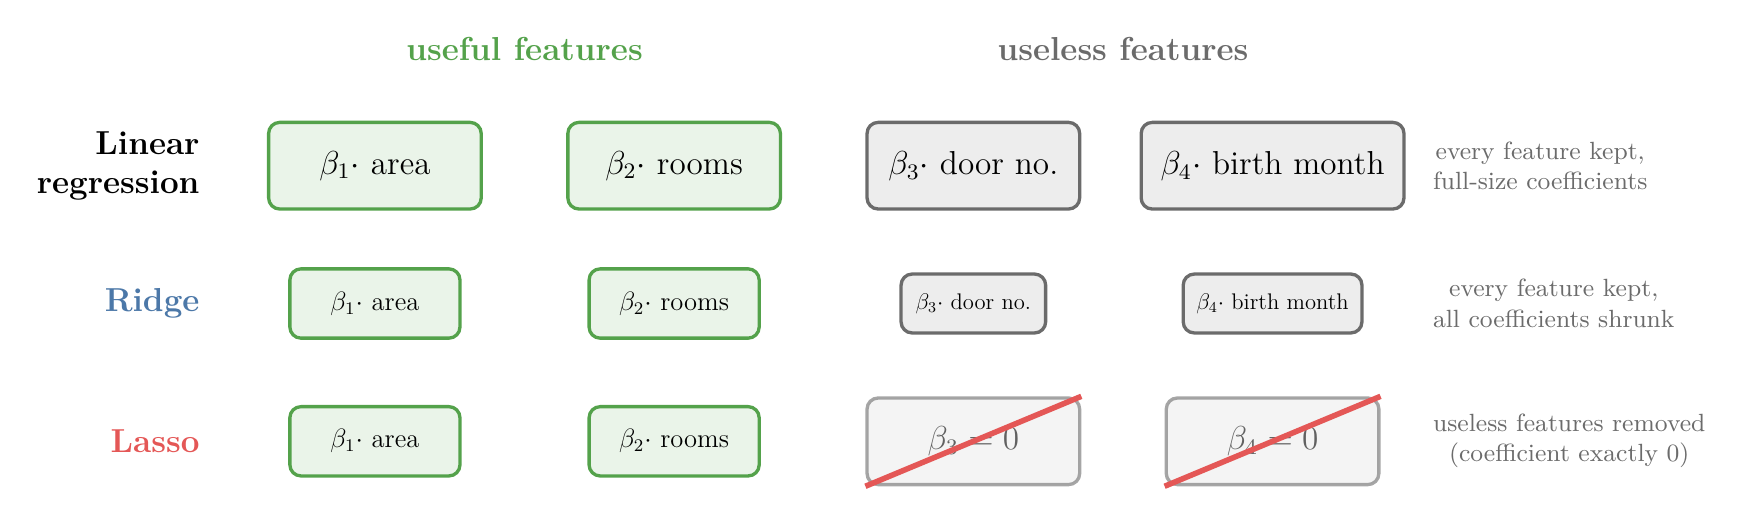
\begin{tikzpicture}[x=3.8cm, y=1.75cm, term/.style={box=#1, minimum width=2.7cm, font=\sffamily\large}]
  \node[font=\sffamily\bfseries\large, text=cgreen] at (1.5,0.85) {useful features};
  \node[font=\sffamily\bfseries\large, text=cgrey] at (3.5,0.85) {useless features};
  % row 1: least squares
  \node[font=\sffamily\bfseries\large, align=right, anchor=east] at (0.45,0) {Linear\\regression};
  \node[term=cgreen] at (1,0) {$\beta_1 \cdot$ area};
  \node[term=cgreen] at (2,0) {$\beta_2 \cdot$ rooms};
  \node[term=cgrey] at (3,0) {$\beta_3 \cdot$ door no.};
  \node[term=cgrey] at (4,0) {$\beta_4 \cdot$ birth month};
  \node[note, anchor=west] at (4.5,0) {every feature kept,\\full-size coefficients};
  % row 2: Ridge
  \node[font=\sffamily\bfseries\large, text=cblue, anchor=east] at (0.45,-1) {Ridge};
  \node[term=cgreen, scale=0.8] at (1,-1) {$\beta_1 \cdot$ area};
  \node[term=cgreen, scale=0.8] at (2,-1) {$\beta_2 \cdot$ rooms};
  \node[term=cgrey, scale=0.68] at (3,-1) {$\beta_3 \cdot$ door no.};
  \node[term=cgrey, scale=0.68] at (4,-1) {$\beta_4 \cdot$ birth month};
  \node[note, anchor=west] at (4.5,-1) {every feature kept,\\all coefficients shrunk};
  % row 3: Lasso
  \node[font=\sffamily\bfseries\large, text=cred, anchor=east] at (0.45,-2) {Lasso};
  \node[term=cgreen, scale=0.8] at (1,-2) {$\beta_1 \cdot$ area};
  \node[term=cgreen, scale=0.8] at (2,-2) {$\beta_2 \cdot$ rooms};
  \node[term=cgrey, opacity=0.6] (a) at (3,-2) {$\beta_3 = 0$};
  \node[term=cgrey, opacity=0.6] (b) at (4,-2) {$\beta_4 = 0$};
  \draw[cred, line width=2pt] (a.south west) -- (a.north east) (b.south west) -- (b.north east);
  \node[note, anchor=west] at (4.5,-2) {useless features removed\\(coefficient exactly 0)};
\end{tikzpicture}
\end{document}
